\documentclass[a4paper,12pt]{jsarticle}

\usepackage[dvipdfmx]{graphicx,color}

\usepackage[T1]{fontenc}
\usepackage{lmodern}

\usepackage{amsmath}
\usepackage{newtxmath,newtxtext}
\usepackage{bm}

\usepackage{here}

\usepackage[dvipdfmx]{hyperref}
\usepackage{pxjahyper}
\hypersetup{
  setpagesize=false,
  bookmarksnumbered=true,
  pdftitle={吾輩は猫である},
  pdfauthor={夏目 漱石},
  colorlinks=true
}

\title{吾輩は猫である}
\author{夏目 漱石}
\date{1905年10月6日}

\begin{document}

\maketitle

吾輩は猫(図\ref{fig:cat})である\cite{natsume1905wagahai}。
名前はまだ無い。
\begin{align}
  f(\bm{x}; \bm{\mu}, \mathbf{\Sigma})
  =
  \frac{1}{{(2 \pi)}^{k / 2} \sqrt{|\mathbf{\Sigma}|}}
  \exp \left[ -\frac{(\bm{x} - \bm{\mu})^\top \mathbf{\Sigma}^{-1} (\bm{x} - \bm{\mu})}{2} \right]
\end{align}

\begin{figure}[H]
  \centering
  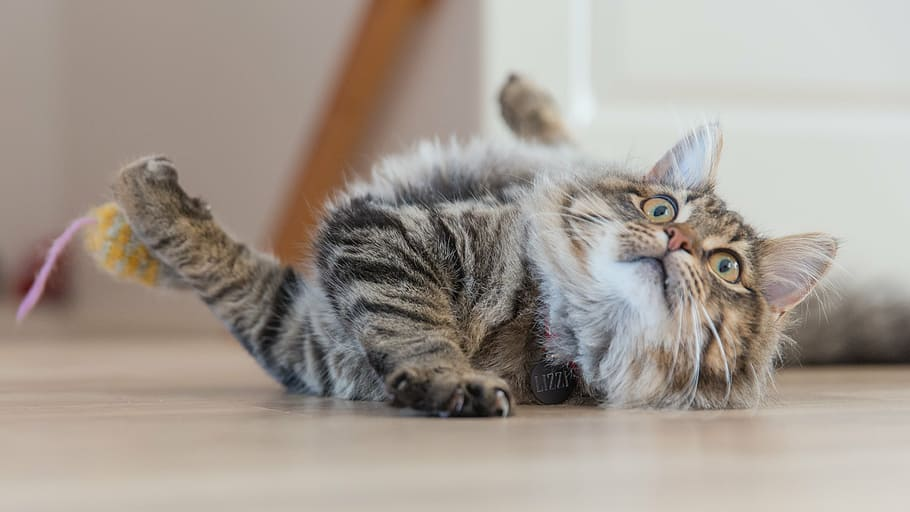
\includegraphics[width=10.0cm]{figs/cat.jpg}
  \caption{猫\protect\footnotemark[1]}
  \label{fig:cat}
\end{figure}

\footnotetext[1]{License: \href{https://creativecommons.org/publicdomain/zero/1.0/}{Creative Commons Zero}}

\bibliographystyle{jplain}
\bibliography{main}

\end{document}
